\chapter{Industry-Level Analysis: Einzelhandel / Branchenebene-Analyse: Einzelhandel / 行业层面分析：零售业}

\section{German Retail Industry Overview / Überblick über die deutsche Einzelhandelsbranche / 德国零售业概述}

\begin{otherlanguage}{ngerman}
Der deutsche Einzelhandel (Einzelhandel) ist einer der größten und wettbewerbsintensivsten Märkte Europas:
\begin{itemize}
    \item Marktvolumen: über 500 Milliarden Euro
    \item Hauptakteure: Edeka, Rewe, Aldi, Lidl, Kaufland
    \item Struktur: Mix aus Discountern, Supermärkten und Hypermarkets
    \item Trends: Digitalisierung, Nachhaltigkeit, Convenience
\end{itemize}
\end{otherlanguage}

The German retail industry (Einzelhandel) is one of the largest and most competitive markets in Europe:
\begin{itemize}
    \item Market volume: over 500 billion euros
    \item Key players: Edeka, Rewe, Aldi, Lidl, Kaufland
    \item Structure: Mix of discounters, supermarkets, and hypermarkets
    \item Trends: Digitalization, sustainability, convenience
\end{itemize}

德国零售业是欧洲最大、竞争最激烈的市场之一：
\begin{itemize}
    \item 市场规模：超过5000亿欧元
    \item 主要参与者：艾德卡、Rewe、Aldi、Lidl、Kaufland
    \item 结构：折扣店、超市和大卖场的混合
    \item 趋势：数字化、可持续性、便利性
\end{itemize}

\section{Market Structure / Marktstruktur / 市场结构}

\begin{otherlanguage}{ngerman}
\begin{table}[h]
\centering
\begin{tabular}{lcc}
\toprule
\textbf{Unternehmen} & \textbf{Marktanteil (\%)} & \textbf{Umsatz (Mrd. €)} \\
\midrule
Edeka & 26.0 & 60+ \\
Rewe & 15.0 & 35+ \\
Aldi & 12.0 & 28+ \\
Lidl & 10.0 & 24+ \\
Kaufland & 8.0 & 18+ \\
\bottomrule
\end{tabular}
\caption{Marktanteile im deutschen Lebensmitteleinzelhandel}
\end{table}
\end{otherlanguage}

% Market Share Pie Chart
\begin{figure}[h]
\centering
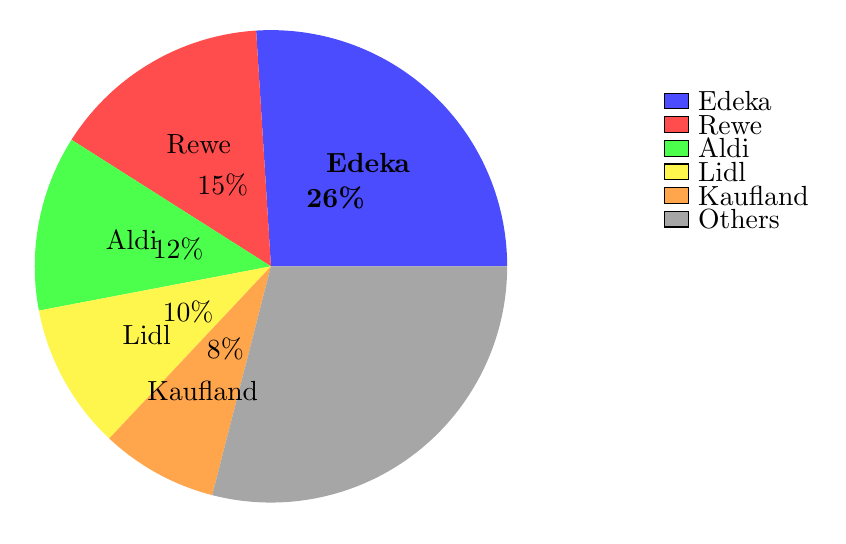
\begin{tikzpicture}
    % Pie chart for market share
    \def\radius{3cm}
    \def\edeka{26}
    \def\rewe{15}
    \def\aldi{12}
    \def\lidl{10}
    \def\kaufland{8}
    \def\others{29}
    
    % Calculate angles
    \pgfmathsetmacro{\edekaAngle}{360*\edeka/100}
    \pgfmathsetmacro{\reweAngle}{360*\rewe/100}
    \pgfmathsetmacro{\aldiAngle}{360*\aldi/100}
    \pgfmathsetmacro{\lidlAngle}{360*\lidl/100}
    \pgfmathsetmacro{\kauflandAngle}{360*\kaufland/100}
    
    % Draw pie slices
    \fill[blue!70] (0,0) -- (0:\radius) arc (0:\edekaAngle:\radius) -- cycle;
    \fill[red!70] (0,0) -- (\edekaAngle:\radius) arc (\edekaAngle:{\edekaAngle+\reweAngle}:\radius) -- cycle;
    \fill[green!70] (0,0) -- ({\edekaAngle+\reweAngle}:\radius) arc ({\edekaAngle+\reweAngle}:{\edekaAngle+\reweAngle+\aldiAngle}:\radius) -- cycle;
    \fill[yellow!70] (0,0) -- ({\edekaAngle+\reweAngle+\aldiAngle}:\radius) arc ({\edekaAngle+\reweAngle+\aldiAngle}:{\edekaAngle+\reweAngle+\aldiAngle+\lidlAngle}:\radius) -- cycle;
    \fill[orange!70] (0,0) -- ({\edekaAngle+\reweAngle+\aldiAngle+\lidlAngle}:\radius) arc ({\edekaAngle+\reweAngle+\aldiAngle+\lidlAngle}:{\edekaAngle+\reweAngle+\aldiAngle+\lidlAngle+\kauflandAngle}:\radius) -- cycle;
    \fill[gray!70] (0,0) -- ({\edekaAngle+\reweAngle+\aldiAngle+\lidlAngle+\kauflandAngle}:\radius) arc ({\edekaAngle+\reweAngle+\aldiAngle+\lidlAngle+\kauflandAngle}:360:\radius) -- cycle;
    
    % Labels
    \node at ({\edekaAngle/2}:\radius*0.6) {\textbf{Edeka}};
    \node at ({\edekaAngle/2}:\radius*0.4) {\textbf{26\%}};
    \node at ({\edekaAngle+\reweAngle/2}:\radius*0.6) {Rewe};
    \node at ({\edekaAngle+\reweAngle/2}:\radius*0.4) {15\%};
    \node at ({\edekaAngle+\reweAngle+\aldiAngle/2}:\radius*0.6) {Aldi};
    \node at ({\edekaAngle+\reweAngle+\aldiAngle/2}:\radius*0.4) {12\%};
    \node at ({\edekaAngle+\reweAngle+\aldiAngle+\lidlAngle/2}:\radius*0.6) {Lidl};
    \node at ({\edekaAngle+\reweAngle+\aldiAngle+\lidlAngle/2}:\radius*0.4) {10\%};
    \node at ({\edekaAngle+\reweAngle+\aldiAngle+\lidlAngle+\kauflandAngle/2}:\radius*0.6) {Kaufland};
    \node at ({\edekaAngle+\reweAngle+\aldiAngle+\lidlAngle+\kauflandAngle/2}:\radius*0.4) {8\%};
    
    % Legend
    \begin{scope}[xshift=5cm, yshift=2cm]
        \draw[fill=blue!70] (0,0) rectangle (0.3,0.2);
        \node[right] at (0.3,0.1) {Edeka};
        \draw[fill=red!70] (0,-0.3) rectangle (0.3,-0.1);
        \node[right] at (0.3,-0.2) {Rewe};
        \draw[fill=green!70] (0,-0.6) rectangle (0.3,-0.4);
        \node[right] at (0.3,-0.5) {Aldi};
        \draw[fill=yellow!70] (0,-0.9) rectangle (0.3,-0.7);
        \node[right] at (0.3,-0.8) {Lidl};
        \draw[fill=orange!70] (0,-1.2) rectangle (0.3,-1.0);
        \node[right] at (0.3,-1.1) {Kaufland};
        \draw[fill=gray!70] (0,-1.5) rectangle (0.3,-1.3);
        \node[right] at (0.3,-1.4) {Others};
    \end{scope}
\end{tikzpicture}
\caption{Market Share Distribution / Marktanteilsverteilung / 市场份额分布}
\end{figure}

\begin{table}[h]
\centering
\begin{tabular}{lcc}
\toprule
\textbf{Company} & \textbf{Market Share (\%)} & \textbf{Revenue (Billion €)} \\
\midrule
Edeka & 26.0 & 60+ \\
Rewe & 15.0 & 35+ \\
Aldi & 12.0 & 28+ \\
Lidl & 10.0 & 24+ \\
Kaufland & 8.0 & 18+ \\
\bottomrule
\end{tabular}
\caption{Market shares in German food retail}
\end{table}

\begin{table}[h]
\centering
\begin{tabular}{lcc}
\toprule
\textbf{公司} & \textbf{市场份额 (\%)} & \textbf{收入（十亿欧元）} \\
\midrule
艾德卡 & 26.0 & 60+ \\
Rewe & 15.0 & 35+ \\
Aldi & 12.0 & 28+ \\
Lidl & 10.0 & 24+ \\
Kaufland & 8.0 & 18+ \\
\bottomrule
\end{tabular}
\caption{德国食品零售市场份额}
\end{table}

\section{Industry Trends / Branchentrends / 行业趋势}

\begin{otherlanguage}{ngerman}
\begin{itemize}
    \item \textbf{Digitalisierung}: E-Commerce, Click \& Collect, Mobile Apps
    \item \textbf{Nachhaltigkeit}: Bio-Produkte, CO2-Reduktion, Verpackungsreduktion
    \item \textbf{Convenience}: Kleinere Läden in Innenstädten, 24/7-Verfügbarkeit
    \item \textbf{Preisdruck}: Starker Wettbewerb durch Discounter
\end{itemize}
\end{otherlanguage}

\begin{itemize}
    \item \textbf{Digitalization}: E-commerce, click \& collect, mobile apps
    \item \textbf{Sustainability}: Organic products, CO2 reduction, packaging reduction
    \item \textbf{Convenience}: Smaller stores in city centers, 24/7 availability
    \item \textbf{Price pressure}: Strong competition from discounters
\end{itemize}

\begin{itemize}
    \item \textbf{数字化}：电子商务、点击取货、移动应用
    \item \textbf{可持续性}：有机产品、二氧化碳减排、包装减少
    \item \textbf{便利性}：市中心的小型商店、24/7可用性
    \item \textbf{价格压力}：来自折扣店的激烈竞争
\end{itemize}
